\documentclass{beamer}
\usetheme{Madrid}
\usecolortheme{default}

\usepackage[utf8]{inputenc}
\usepackage{amsmath}
\usepackage{amsfonts}
\usepackage{amssymb}
\usepackage{graphicx}
\usepackage{tikz}
\usetikzlibrary{arrows.meta, shapes.geometric, positioning, chains}

% Custom colors for the nodes
\definecolor{extcolor}{RGB}{230, 230, 230}
\definecolor{branchcolor}{RGB}{245, 245, 245}
\definecolor{leafcolor}{RGB}{255, 255, 255}
\definecolor{highlightred}{RGB}{200, 0, 0}

\title{Stateless Ethereum: From MPT to Verkle Tries}
\subtitle{Thesis Helper Presentation}

\date{\today}

\begin{document}

\maketitle
% --- New Basic Intro Section ---

\begin{frame}{What is Blockchain?}
\begin{itemize}
    \item A blockchain is a shared digital record that is maintained by many computers together.
    \item It stores information in \textbf{blocks}, and these blocks are connected one after another.
    \item Each new block is linked to the previous one using cryptography, so changing old data becomes very difficult.
    \item This helps many participants trust the same record, even without a central authority.
\end{itemize}

\vspace{0.3cm}
\textbf{In simple words:} Blockchain is a shared and hard-to-tamper digital ledger.
\end{frame}

\begin{frame}{What is Ethereum?}
\begin{itemize}
    \item Ethereum is a blockchain platform, but it does more than just record payments.
    \item It can also run \textbf{smart contracts}, which are programs stored on the blockchain.
    \item These smart contracts automatically execute when certain transactions or conditions occur.
    \item So, Ethereum is not only for transferring money; it also supports decentralized applications.
\end{itemize}

\vspace{0.3cm}
\textbf{In short:} Ethereum is a programmable blockchain.
\end{frame}

\begin{frame}{What is the Ethereum State?}
\begin{block}{Definition}
The \textbf{Ethereum state} is the latest snapshot of all accounts and their current data.
\end{block}

\begin{itemize}
    \item It shows the current condition of the network at a specific moment.
    \item It tells us things like \textbf{who has how much balance} and \textbf{what data a smart contract currently stores}.
    \item Whenever a valid transaction is executed, this state gets updated.
    \item So Ethereum does not only keep transaction history; it also keeps track of the latest outcome of that history.
\end{itemize}

\vspace{0.2cm}
\textbf{Examples of state data:}
\begin{itemize}
    \item Account balance
    \item Nonce
    \item Contract code
    \item Contract storage
\end{itemize}
\end{frame}

\begin{frame}{Types of Accounts in Ethereum}
\begin{columns}[t]
\column{0.48\textwidth}
\textbf{Externally Owned Account (EOA)}
\begin{itemize}
    \item Controlled by a user through a private key
    \item Used by normal users
    \item Can send transactions
    \item Stores balance and nonce
\end{itemize}

\column{0.48\textwidth}
\textbf{Contract Account}
\begin{itemize}
    \item Controlled by smart contract code
    \item Executes logic automatically
    \item Stores balance, code, and storage data
    \item Used to run decentralized applications
\end{itemize}
\end{columns}

\vspace{0.3cm}
\textbf{Simple idea:} EOAs are user accounts, while contract accounts are program accounts.
\end{frame}

\begin{frame}{How State Changes}
\textbf{Ethereum follows a state transition process:}

\[
\text{Current State} + \text{Transaction} \rightarrow \text{New State}
\]

\begin{itemize}
    \item First, a user sends a transaction.
    \item Then Ethereum processes that transaction according to its rules.
    \item As a result, balances, nonces, or contract storage may change.
    \item After execution, the network moves from the old state to a new updated state.
\end{itemize}

\vspace{0.3cm}
\textbf{Example:}
\begin{itemize}
    \item Alice sends 1 ETH to Bob
    \item Alice's balance decreases
    \item Bob's balance increases
    \item Alice's nonce increases by 1
\end{itemize}
\end{frame}

\begin{frame}{Why Do We Need a State Root?}
\begin{itemize}
    \item Ethereum state is very large because it contains millions of accounts and storage entries.
    \item It is not practical to represent this huge state in a simple list inside every block.
    \item So Ethereum stores a compact cryptographic summary of the whole state, called the \textbf{State Root}.
    \item This state root is included in the block header.
    \item If even a small part of the state changes, the state root also changes.
\end{itemize}

\vspace{0.3cm}
\begin{block}{Why this is important}
The state root gives one compact fingerprint of the entire Ethereum state.
\end{block}
\end{frame}

\begin{frame}{Why a Tree Structure is Needed}
A simple database is not enough for Ethereum.

\begin{itemize}
    \item We need to find accounts and storage values efficiently
    \item We need a secure way to prove that a value is correct
    \item We need one compact root that represents the whole state
\end{itemize}

\vspace{0.3cm}
\textbf{That is why Ethereum uses a tree-based authenticated data structure called:}
\begin{center}
\textbf{Merkle Patricia Trie (MPT)}
\end{center}
\end{frame}

\end{frame}
% --- Slide 1: Current State Trie (MPT) ---
% \begin{frame}{1.1 The Ethereum State: Merkle Patricia Trie (MPT)}
% The Ethereum State is a mapping of \textbf{Addresses} to \textbf{Account States}. It uses a modified Merkle Patricia Trie.
%     \begin{itemize}
%         \item \textbf{Merkle Tree:} Provides cryptographic integrity.
%         \item \textbf{Patricia Trie:} Provides efficient key-value lookups.
%     \end{itemize}
    
%     \vspace{0.3cm}
%     Consider the following key-value pairs:
%     \begin{center}
%     \begin{tabular}{|l|l|}
%         \hline
%         \textbf{Key} & \textbf{Value} \\ \hline
%         \texttt{1111} & ahoj \\
%         \texttt{11110AA} & hi \\
%         \texttt{11112FF} & thus \\ \hline
%     \end{tabular}
%     \end{center}
% \end{frame}

% PROBLEM 1
% The diagrams and tables are out of order in the next 3 frames. Have to bring them in order for better explanation. These diagrams and tables are available in the paper I gave you

\begin{frame}{1.1 The Ethereum State: Merkle Patricia Trie (MPT)}
The Ethereum State is a mapping of \textbf{Addresses} to \textbf{Account States}. It uses a modified Merkle Patricia Trie.
    The MPT is a combination of a \textbf{Patricia Trie} and a \textbf{Merkle Tree} .
    \begin{itemize}
        \item \textbf{Patricia Trie (Prefix Tree):} Keys are paths. Nodes share common prefixes to save space.
        \item \textbf{Merkle Logic:} Every node is identified by the \textbf{Keccak-256 hash} of its contents. A change in a leaf ripples up to the \textbf{State Root}.
        \item \textbf{Hexary Structure:} In Ethereum, each "nibble" (4 bits) represents a hex character (0-F), leading to a 16-way branching factor.
    \end{itemize}
    % \centering
    % \begin{tikzpicture}[scale=0.8, every node/.style={scale=0.8}, >=Stealth]
    %     \node[draw, circle] (root) {Root Hash};
    %     \node[draw, rectangle, below of=root, node distance=1.2cm, fill=blue!5] (path) {Shared Prefix: "0x1111"};
    %     \draw[->] (root) -- (path);
        
    %     \node[draw, rectangle, below of=path, node distance=1.5cm, fill=orange!10] (branch) {Branch [0...F]};
    %     \draw[->] (path) -- (branch);
        
    %     \node[draw, rectangle, below left of=branch, xshift=-1cm, yshift=-0.5cm, fill=green!5] (L1) {Leaf: Value A};
    %     \node[draw, rectangle, below right of=branch, xshift=1cm, yshift=-0.5cm, fill=green!5] (L2) {Leaf: Value B};
        
    %     \draw[->] (branch) -- (L1) node[midway, left] {nibble '0'};
    %     \draw[->] (branch) -- (L2) node[midway, right] {nibble 'A'};
    % \end{tikzpicture}
\end{frame}

% \begin{frame}{1.2 MPT Structure}
%      \centering
%     \begin{tikzpicture}[scale=0.8, every node/.style={scale=0.8}, >=Stealth]
%         \node[draw, circle] (root) {Root Hash};
%         \node[draw, rectangle, below of=root, node distance=1.2cm, fill=blue!5] (path) {Shared Prefix: "0x1111"};
%         \draw[->] (root) -- (path);
        
%         \node[draw, rectangle, below of=path, node distance=1.5cm, fill=orange!10] (branch) {Branch [0...F]};
%         \draw[->] (path) -- (branch);
        
%         \node[draw, rectangle, below left of=branch, xshift=-1cm, yshift=-0.5cm, fill=green!5] (L1) {Leaf: Value A};
%         \node[draw, rectangle, below right of=branch, xshift=1cm, yshift=-0.5cm, fill=green!5] (L2) {Leaf: Value B};
        
%         \draw[->] (branch) -- (L1) node[midway, left] {nibble '0'};
%         \draw[->] (branch) -- (L2) node[midway, right] {nibble 'A'};
%     \end{tikzpicture}
% \end{frame}

\begin{frame}{1.2 MPT Structure}
\begin{columns}[t]
    \begin{column}{0.5\textwidth}
    Consider the following keys:
    \vspace{0.3cm}
    \begin{tabular}{l}
        \textbf{Keys} \\ \hline
        \texttt{110} \\
        \texttt{1100} \\
        \texttt{11011} \\
        \texttt{11110} \\ 
    \end{tabular}
    \pause
    \begin{itemize}
        Simple Prefix tree
        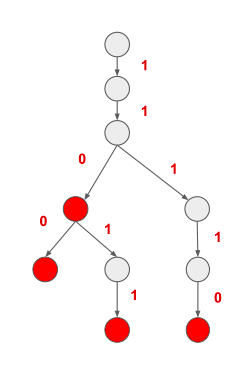
\includegraphics[width=0.5\textwidth]{prefix_tree.png}
    \end{itemize}
    % 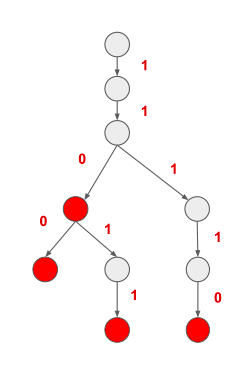
\includegraphics[width=0.5\textwidth]{prefix_tree.png}
    \end{column}
    \pause
    \begin{column}{0.5\textwidth}
    Merkle tree using this prefix tree
    \vspace{0.3cm}
    \begin{center}
        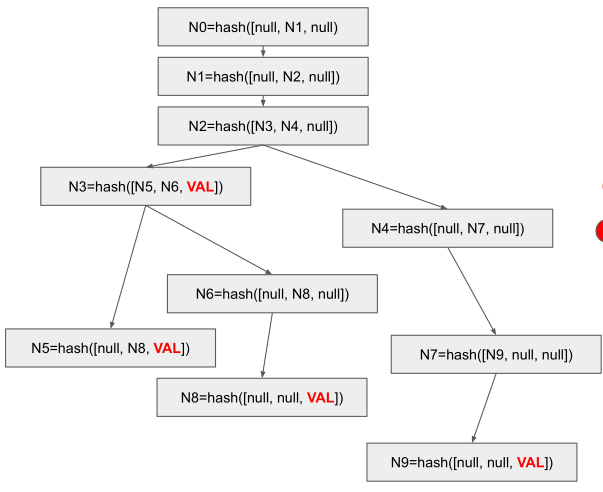
\includegraphics[width=\textwidth]{merkle_tree.png}
    \end{center}
    \end{column}
\end{columns}
\end{frame}

\begin{frame}{1.2 MPT Structure}
    \begin{columns}[t]
       \begin{column}{0.5\textwidth}
           Patricia trie with path compression
           \vspace{0.3cm}
            \begin{center}
                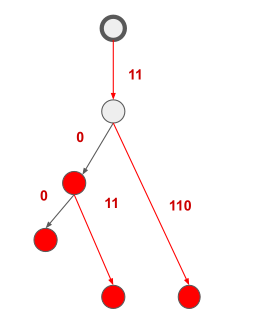
\includegraphics[width=0.75\textwidth]{patricia_trie.png}
            \end{center}
       \end{column}
       \begin{column}{0.5\textwidth}
           Merkle Patricia Trie (MPT)
           \vspace{0.3cm}
            \begin{center}
                \includegraphics[width=0.75\textwidth]{mpt.png}
            \end{center}
       \end{column}
    \end{columns}
\end{frame}

% --- Slide 1.3: MPT Node Anatomy ---
\begin{frame}{1.3 Anatomy of MPT Nodes}
    To implement the path compression strategy of patricia, MPT uses three specific node types:
    \vspace{0.3cm}
    
    % \centering
    % \begin{tikzpicture}[node distance=0.8cm, every node/.style={font=\scriptsize}]
        
    %     % Extension Node
    %     \node[fill=extcolor, draw, minimum width=5cm] (extH) {\textbf{Extension Node}};
    %     \node[draw, below=0pt of extH, minimum width=1.5cm] (ext1) {Prefix: -};
    %     \node[draw, right=0pt of ext1, minimum width=2cm] (ext2) {\textcolor{highlightred}{Shared: 1111}};
    %     \node[draw, right=0pt of ext2, minimum width=1.5cm] (ext3) {Next Hash};
        
    %     % Branch Node
    %     \node[fill=branchcolor, draw, minimum width=5cm, below=1.2cm of extH] (brH) {\textbf{Branch Node}};
    %     \node[draw, below=0pt of brH, minimum width=3.5cm] (br1) {$v_0, v_1, \dots, \mathbf{\textcolor{highlightred}{v_2}}, \dots, v_{15}$};
    %     \node[draw, right=0pt of br1, minimum width=1.5cm] (br2) {Value: \textbf{ahoj}};
        
    %     % Leaf Nodes
    %     \node[fill=leafcolor, draw, minimum width=4cm, below left=1.2cm and -1cm of brH] (lf1H) {\textbf{Leaf Node (hi)}};
    %     \node[draw, below=0pt of lf1H, minimum width=1.5cm] (lf1a) {Prefix: 10};
    %     \node[draw, right=0pt of lf1a, minimum width=1.5cm] (lf1b) {\textcolor{highlightred}{Suffix: AA}};
    %     \node[draw, right=0pt of lf1b, minimum width=1cm] (lf1c) {hi};

    %     \node[fill=leafcolor, draw, minimum width=4cm, below right=1.2cm and -1cm of brH] (lf2H) {\textbf{Leaf Node (thus)}};
    %     \node[draw, below=0pt of lf2H, minimum width=1.5cm] (lf2a) {Prefix: 10};
    %     \node[draw, right=0pt of lf2a, minimum width=1.5cm] (lf2b) {\textcolor{highlightred}{Suffix: FF}};
    %     \node[draw, right=0pt of lf2b, minimum width=1cm] (lf2c) {thus};

    %     % Connections
    %     \draw[->, thick] (ext3.south) -- (brH.north);
    %     \draw[->] (br1.south) -- (lf1H.north);
    %     \draw[->] (br1.south) -- (lf2H.north);
    % \end{tikzpicture}
    \begin{center}
        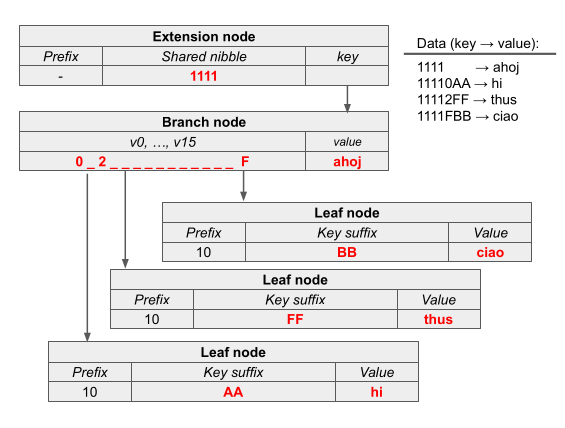
\includegraphics[width=0.75\textwidth]{mpt_nodes.png}
    \end{center}
    % \vspace{0.3cm}
    % \begin{itemize}
    %     \item \textbf{Extension:} Collapses multiple nodes with a single child into one.
    %     \item \textbf{Branch:} A 17-item list (16 pointers + 1 optional value).
    %     \item \textbf{Leaf:} Stores the remaining part of the key (\textit{suffix}) and the final value.
    % \end{itemize}
\end{frame}
\begin{frame}{1.3 Anatomy of MPT Nodes}
    \vspace{0.3cm}
    \begin{itemize}
        \item \textbf{Extension:} Collapses multiple nodes with a single child into one.
        \item \textbf{Branch:} A 17-item list (16 pointers + 1 optional value).
        \item \textbf{Leaf:} Stores the remaining part of the key (\textit{suffix}) and the final value.
    \end{itemize}
\end{frame}
% --- Slide 2: Problems of Stateful Ethereum ---
\begin{frame}{2. The Problems of Stateful Ethereum}
    Currently, all clients must be "Stateful" (storing the full state).
    \begin{block}{The "State Bloat" Issue}
        \begin{itemize}
            \item \textbf{Storage Requirements:} The state grows linearly over time (currently hundreds of GBs).
            \item \textbf{Hardware Barrier:} High SSD requirements prevent hobbyists from running full nodes.
            \item \textbf{Sync Time:} New nodes take days or weeks to synchronize.
            \item \textbf{Centralization Risk:} Only large data centers can afford the overhead. Which violates the fundamental principal of blockchain which is decentralization
        \end{itemize}
    \end{block}
\end{frame}

% --- Slide 3: Shifting to Statelessness ---
\begin{frame}{3. Shifting to Stateless Ethereum}
    \textbf{Core Concept:} Nodes need not store the entire state to verify a block.
    \begin{itemize}
        \item \textbf{Witnesses:} Transactions come bundled with a "Proof" (Witness).
        \item \textbf{Verification:} A node uses the current \textbf{State Root} and the \textbf{Witness} to verify that the balance/nonce change is valid without looking at the local disk.
    \end{itemize}
\end{frame}

% --- Slide 4: Problems with MPT Proofs ---

% PROBLEM 2
% The main demerit is 'witness contains all the hashes of the siblings along the path from the leaf to the root'. Have to explain this using diagrams

\begin{frame}{4. The Demerits of MPT Proofs}
    Can we use MPT for statelessness?
    \pause
    \vspace{0.2cm}
    % \begin{center}
    %     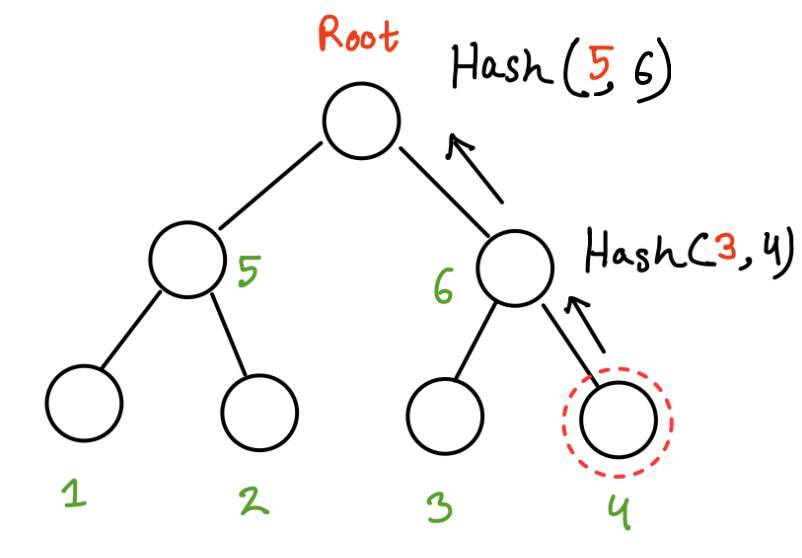
\includegraphics[width=0.4\textwidth]{image1.png}
        
    %     \textit{\small Witness contains all the hashes of the siblings along the path}
    % \end{center}
    \vspace{0.3cm}
    \centering
    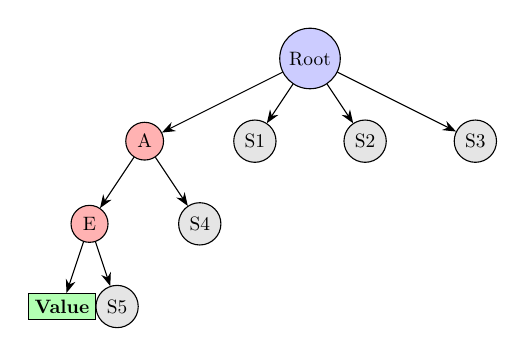
\begin{tikzpicture}[scale=0.7, every node/.style={scale=0.7}, >=Stealth]
        % Root
        \node[draw, circle, fill=blue!20] (root) at (0,0) {Root};
        
        % Level 1
        \node[draw, circle, fill=red!30] (A) at (-3,-1.5) {A};
        \node[draw, circle, fill=gray!20] (B) at (-1,-1.5) {S1};
        \node[draw, circle, fill=gray!20] (C) at (1,-1.5) {S2};
        \node[draw, circle, fill=gray!20] (D) at (3,-1.5) {S3};
        
        % Level 2
        \node[draw, circle, fill=red!30] (E) at (-4,-3) {E};
        \node[draw, circle, fill=gray!20] (F) at (-2,-3) {S4};
        
        % Leaf
        \node[draw, rectangle, fill=green!30] (leaf) at (-4.5,-4.5) {\textbf{Value}};
        \node[draw, circle, fill=gray!20] (S5) at (-3.5,-4.5) {S5};
        
        % Edges
        \draw[->] (root) -- (A);
        \draw[->] (root) -- (B);
        \draw[->] (root) -- (C);
        \draw[->] (root) -- (D);
        \draw[->] (A) -- (E);
        \draw[->] (A) -- (F);
        \draw[->] (E) -- (leaf);
        \draw[->] (E) -- (S5);
    \end{tikzpicture}
    
    \vspace{0.3cm}
    \textbf{Proof Contains:} Path nodes (red) + All sibling nodes (gray, S1-S5). \textbf{Result:} Proof size grows with tree depth. For depth $d$ and branching factor 16: $\sim d \times 15 \times 32$ bytes $\approx$ 3-6 KB per proof.
    \pause
    \begin{center}
    \textcolor{red}{\textbf{In short, Witness contains all the hashes of the siblings along the path}}
    \end{center}
    % \begin{itemize}
    %     \item \textbf{Witness Size:} MPT is a hexary trie ($16$-way). The number of sibling hashes required for a proof is massive.
    %     \item \textbf{Bandwidth:} Average block witnesses in MPT would be $\sim 1-3$ MB. This is too heavy for the p2p network to propagate every $12$ seconds.
    %     \item \textbf{Proof Complexity:} Verification requires many rounds of hashing (Keccak256).
    % \end{itemize}
\end{frame}

% --- Slide 5: Verkle Tries ---

% PROBLEM 3
% Need better diagrams and clear explanations for verkle trie

\begin{frame}{5.1 Verkle Trie: A Solution}
    \textbf{The Problem:} MPT witnesses are too large ($\sim$2 MB/block) due to 16-way branching requiring many sibling hashes.
    
    \vspace{0.3cm}
    \textbf{Verkle Tree Solution:} Uses vector commitment scheme instead of hashing which enables proving a node without its siblings.
    
    \begin{itemize}
        \item \textbf{Wider Branching:} 256 children per node (vs 16 in MPT) $\rightarrow$ Shallower tree
        \item \textbf{Shorter Proofs:} Using polynomial commitments, Verkle provides a proving method that only needs vector commitment of parent node
    \end{itemize}
\end{frame}

\begin{frame}{5.2 Verkle Tree Structure}
    \begin{center}
        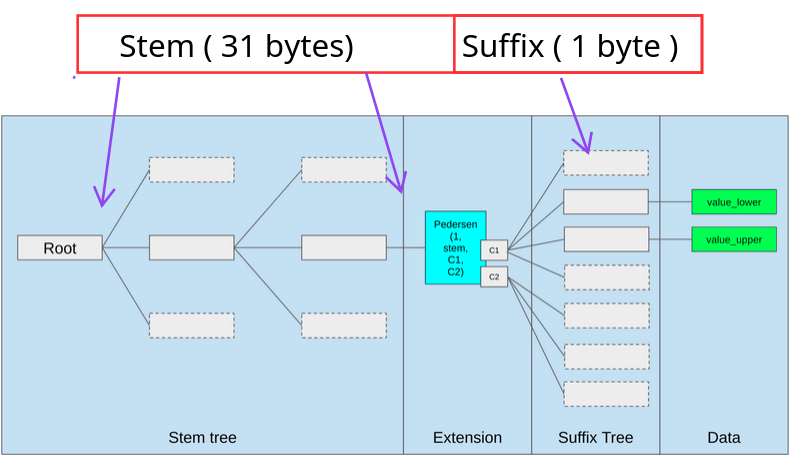
\includegraphics[width=0.8\textwidth]{verkle_tree_struct.png}
    \end{center}
    
    % \begin{itemize}
    %     \item 32 byte key
    %     \item consisting of a 31-byte stem and a 1-byte suffix. The suffix allows 256 children. 
    %     \item Each of these children is divided into two parts resulting in 512 values. Two commitments C1, C2 are calculated for 256 values each
    %     \item Then pedersen hash is calculated from 1, stem, C1 and C2 which is ultimately stored as stem data
    % \end{itemize}
\end{frame}

\begin{frame}{5.2 Verkle Tree Structure}
    \begin{itemize}
        \item 32 byte key
        \item consisting of a 31-byte stem and a 1-byte suffix. The suffix allows 256 children. 
        \begin{center}
            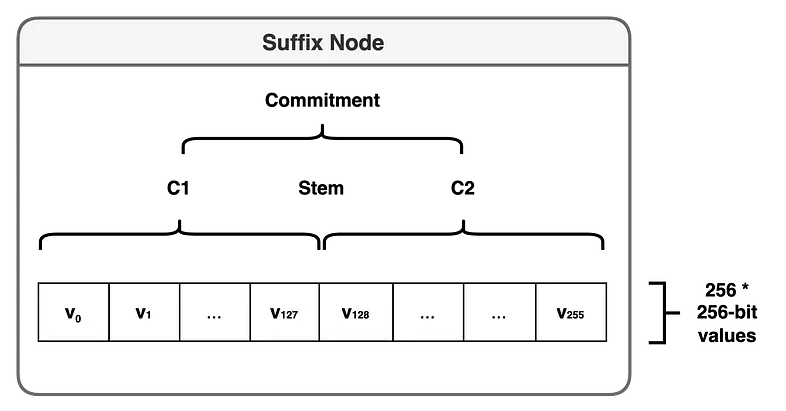
\includegraphics[width=0.8\textwidth]{suffix_node.png}
        \end{center}
    \end{itemize}
\end{frame}

\begin{frame}{5.2 Verkle Tree Structure}
    \begin{itemize}
        \item Each of these children is divided into two parts resulting in 512 values. Two commitments C1, C2 are calculated for 256 values each
        \begin{center}
            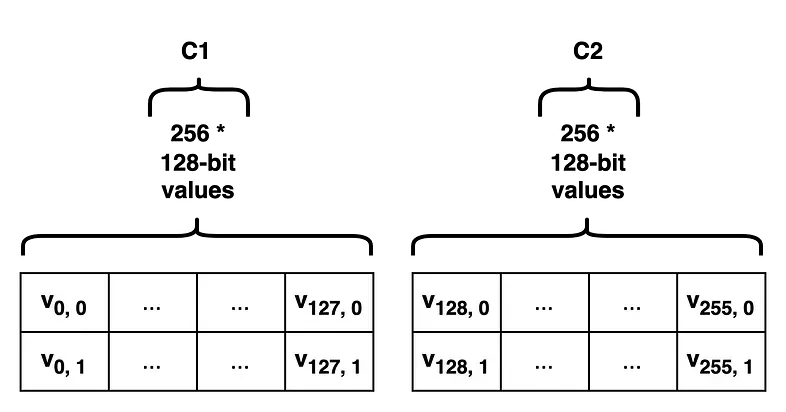
\includegraphics[width=0.8\textwidth]{C1_C2.png}
        \end{center}
        \item Then pedersen hash is calculated from 1, stem, C1 and C2 which is ultimately stored as stem data
    \end{itemize}
\end{frame}

\begin{frame}{5.2 Verkle Tree Structure}
    \begin{itemize}
        \item Inner node holds the stem value of the tree key and stores 256 pointers to sub-nodes
        \begin{center}
            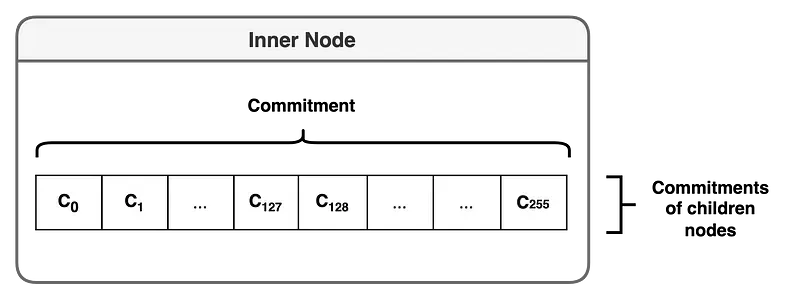
\includegraphics[width=0.8\textwidth]{inner_node.png}
        \end{center}
        \item C0, C1 … C255 represent the commitments of sub-nodes, and the inner node contains these commitments.
    \end{itemize}
\end{frame}

\begin{frame}{5.3 An example of verkle trie}
    An example of verkle tree containing 4 tree keys:
    \begin{itemize}
        \item 0x00..20
        \item 0xdefe…64
        \item 0xde03a8..02
        \item 0xde03a8..ff
    \end{itemize}
    \begin{center}
        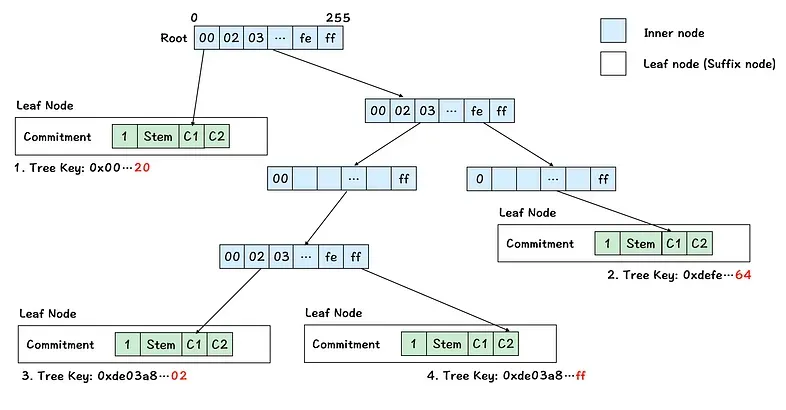
\includegraphics[width=0.7\textwidth]{verkle_trie_example.png}
    \end{center}
\end{frame}

% --- Slide 6: Vector Commitments & ZK Intro ---

% PROBLEM 4
% Need more detail for vector commitments

% filepath: /home/raizen/Documents/Thesis/Experimentation/main.tex

% Replace from line starting with "\begin{frame}{6.1 Vector Commitments..." to end

\begin{frame}{6.1 Vector Commitments: The Core Idea}
    \textbf{Problem with Merkle Trees:} To prove a value, you need \textcolor{red}{all sibling hashes} along the path.
    
    \vspace{0.3cm}
    \textbf{Vector Commitment Solution:} Commit to a vector $(v_0, v_1, \dots, v_{255})$ such that:
    \begin{itemize}
        \item Commitment $C$ is compact (single elliptic curve point, 32 bytes)
        \item Can prove any $v_i$ is at position $i$ without revealing others
        \item \textcolor{green!60!black}{No sibling hashes needed!}
        \item Proof size is constant ($\sim$48 bytes per opening)
    \end{itemize}
    
    \pause
    \vspace{0.3cm}
    \textbf{Approach:} Represent the vector as a polynomial, commit to the polynomial using elliptic curves.
    
    \begin{itemize}
        \item Vector: $(v_0, v_1, v_2, \dots, v_{255})$
        \item Polynomial: $f(x)$ where $f(0) = v_0, f(1) = v_1, \dots, f(255) = v_{255}$
        \item Commitment: $C = [f(s)]_1$ (elliptic curve point)
    \end{itemize}
    
    \pause
    \vspace{0.2cm}
    This uses \textbf{KZG (Kate-Zaverucha-Goldberg)} commitment scheme.
\end{frame}

\begin{frame}{6.2 Step 1: Lagrange Interpolation}
    \textbf{Goal:} Create a polynomial that encodes our vector.
    
    \vspace{0.3cm}
    \textbf{Given:} Data points $(0, v_0), (1, v_1), (2, v_2), \dots, (255, v_{255})$
    
    \textbf{Lagrange Interpolation Formula:}
    \[
    f(x) = \sum_{i=0}^{255} v_i \cdot L_i(x)
    \]
    where $L_i(x) = \prod\limits_{\substack{j=0 \\ j \neq i}}^{255} \frac{x - j}{i - j}$ is the Lagrange basis polynomial.
    
    \pause
    \vspace{0.3cm}
    \textbf{Key Property:} The polynomial $f(x)$ passes through all points:
    \[
    f(i) = v_i \quad \text{for all } i \in \{0, 1, 2, \dots, 255\}
    \]
    
    \pause
    \vspace{0.3cm}
    \textbf{Result:} We now have a polynomial of degree $\leq 255$ that encodes our entire vector.
\end{frame}

\begin{frame}{6.3 Step 2: Extract Coefficients Using FFT}
    \textbf{Goal:} Convert polynomial to coefficient form for efficient computation.
    
    \vspace{0.3cm}
    The Lagrange form is hard to work with directly. We need:
    \[
    f(x) = a_0 + a_1 x + a_2 x^2 + \cdots + a_{255} x^{255}
    \]
    
    \pause
    \vspace{0.3cm}
    \textbf{Fast Fourier Transform (FFT):}
    \begin{itemize}
        \item Efficiently extracts coefficients $a_0, a_1, \dots, a_{255}$
        \item Time complexity: $O(n \log n)$ instead of $O(n^2)$
        \item Essential for practical implementation
    \end{itemize}
    
    \pause
    \vspace{0.3cm}
    \textbf{Result:} We now have the coefficients that represent our polynomial:
    \[
    f(x) = \sum_{i=0}^{255} a_i x^i
    \]
\end{frame}

\begin{frame}{6.4 Step 3: Map to Elliptic Curve Space}
    \textbf{Goal:} Create a cryptographic commitment using elliptic curves.
    
    \vspace{0.3cm}
    \textbf{Trusted Setup Phase} (done once, globally):
    \begin{itemize}
        \item Choose random secret $s$ (then \textcolor{red}{destroyed forever!})
        \item Generate elliptic curve points for powers of $s$:
        \[
        G_1, \quad [s]G_1, \quad [s^2]G_1, \quad \dots, \quad [s^{255}]G_1
        \]
        \item These become public parameters (anyone can use them)
        \item Base point: $G_1$ is a generator of the elliptic curve group
    \end{itemize}
    
    \pause
    \vspace{0.3cm}
    \textbf{Why Elliptic Curves?}
    \begin{itemize}
        \item Operations happen in a group with discrete logarithm hardness
        \item Compact representation (32-48 bytes per point)
        \item Efficient pairing operations for verification
    \end{itemize}
\end{frame}

\begin{frame}{6.5 Step 4: Create the Commitment}
    \textbf{Commitment Computation:}
    
    Given polynomial coefficients $a_0, a_1, \dots, a_{255}$, compute:
    \[
    C = a_0 \cdot G_1 + a_1 \cdot [s]G_1 + a_2 \cdot [s^2]G_1 + \cdots + a_{255} \cdot [s^{255}]G_1
    \]
    
    \pause
    This can be written more compactly as:
    \[
    C = \sum_{i=0}^{255} a_i \cdot [s^i]G_1 = [f(s)]_1
    \]
    
    \pause
    \vspace{0.3cm}
    \textbf{Key Properties:}
    \begin{itemize}
        \item $C$ is a \textbf{single elliptic curve point} (32 bytes)
        \item Represents evaluation $f(s)$ in elliptic curve space
        \item No one knows $s$, so commitment cannot be forged
        \item Acts as a cryptographic digest of the entire vector
    \end{itemize}
    
    \pause
    \vspace{0.2cm}
    \textbf{Result:} Commitment $C$ binds to all 256 values in the vector!
\end{frame}

\begin{frame}{6.6 Step 5: Opening Proof (Proving $f(i) = v_i$)}
    \textbf{Goal:} Prove that position $i$ contains value $v_i$ in commitment $C$.
    
    \vspace{0.3cm}
    \textbf{Proof Generation:}
    \begin{enumerate}
        \item Prover knows the full polynomial $f(x)$
        \item Compute quotient polynomial: 
        \[
        q(x) = \frac{f(x) - v_i}{x - i}
        \]
        \item Generate proof as elliptic curve point: $\pi = [q(s)]_1$
    \end{enumerate}
    
    \pause
    \vspace{0.3cm}
    \textbf{Verification:}
    
    Verifier has: $C$ (commitment), $i$ (position), $v_i$ (claimed value), $\pi$ (proof)
    
    Check using elliptic curve pairing:
    \[
    e(C - [v_i]G_1, G_2) = e(\pi, [s]G_2 - [i]G_2)
    \]
    
    If this pairing equation holds, accept that $f(i) = v_i$.
    
    \pause
    \vspace{0.3cm}
    \textbf{Magic:} Proof $\pi$ is constant size ($\sim$48 bytes) regardless of vector size!
\end{frame}

% % --- Slide 7: Verkle Proof Structure ---
% % PROBLEM 5
% % If there is anything left to explain about the structure of verkle trie you can explain it here. Otherwise this frame can be skipped

% \begin{frame}{7. Structure of Verkle Proofs}
%     The magic of Verkle Tries lies in \textbf{Multi-proofs}.
%     \begin{itemize}
%         \item In MPT, you need siblings for \textit{every} step.
%         \item In Verkle, using polynomial commitments, we can create a single proof that covers \textbf{all} nodes along the path.
%         \item \textbf{Constant Size:} Whether the tree is deep or shallow, the proof size for multiple values remains extremely small.
%     \end{itemize}
% \end{frame}

% --- Slide 8: Comparison & Summary ---

% PROBLEM 6
% Explain the tree like proof of merkle tree and linear proof of verkle tree and then compare the merits and demerits

\begin{frame}{8.1 MPT Proof Generation: Tree-like Structure}
    \textbf{How MPT Proves a Value:} Suppose we want to prove a key
    
    % \vspace{0.3cm}
    % \centering
    % \begin{tikzpicture}[scale=0.7, every node/.style={scale=0.7}, >=Stealth]
    %     % Root
    %     \node[draw, circle, fill=blue!20] (root) at (0,0) {Root};
        
    %     % Level 1
    %     \node[draw, circle, fill=red!30] (A) at (-3,-1.5) {A};
    %     \node[draw, circle, fill=gray!20] (B) at (-1,-1.5) {S1};
    %     \node[draw, circle, fill=gray!20] (C) at (1,-1.5) {S2};
    %     \node[draw, circle, fill=gray!20] (D) at (3,-1.5) {S3};
        
    %     % Level 2
    %     \node[draw, circle, fill=red!30] (E) at (-4,-3) {E};
    %     \node[draw, circle, fill=gray!20] (F) at (-2,-3) {S4};
        
    %     % Leaf
    %     \node[draw, rectangle, fill=green!30] (leaf) at (-4.5,-4.5) {\textbf{Value}};
    %     \node[draw, circle, fill=gray!20] (S5) at (-3.5,-4.5) {S5};
        
    %     % Edges
    %     \draw[->] (root) -- (A);
    %     \draw[->] (root) -- (B);
    %     \draw[->] (root) -- (C);
    %     \draw[->] (root) -- (D);
    %     \draw[->] (A) -- (E);
    %     \draw[->] (A) -- (F);
    %     \draw[->] (E) -- (leaf);
    %     \draw[->] (E) -- (S5);
    % \end{tikzpicture}
    
    % \vspace{0.3cm}
    % \textbf{Proof Contains:} Path nodes (red) + All sibling nodes (gray, S1-S5). \textbf{Result:} Proof size grows with tree depth. For depth $d$ and branching factor 16: $\sim d \times 15 \times 32$ bytes $\approx$ 3-6 KB per proof.
    \begin{center}
        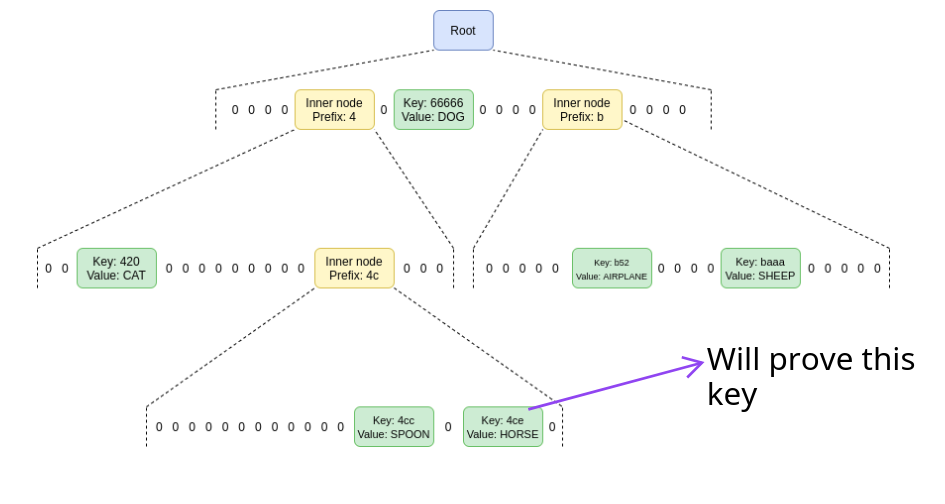
\includegraphics[width=\textwidth]{tree_with_proof_key.png}
    \end{center}
\end{frame}

\begin{frame}{8.1 MPT Proof Generation: Tree-like Structure}
    \textbf{How MPT Proves a Value:} For that we must provide all sibling hashes along the path
    \begin{center}
        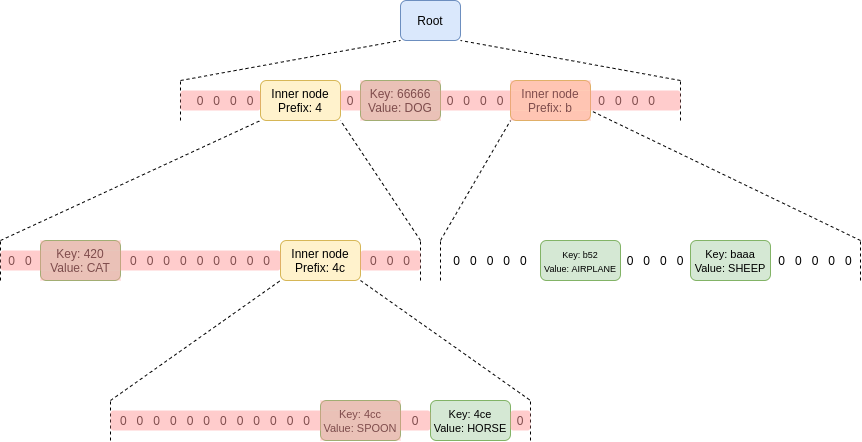
\includegraphics[width=\textwidth]{merkle_proof.png}
    \end{center}
\end{frame}

\begin{frame}{8.2 Verkle Proof Generation: Linear Structure}
    \textbf{How Verkle Proves a Value:} Uses polynomial commitment opening. For the above case, it only needs 3 nodes
    \vspace{0.3cm}
    % \centering
    % \begin{tikzpicture}[scale=0.7, every node/.style={scale=0.7}, >=Stealth]
    %     % Root
    %     \node[draw, rectangle, rounded corners, fill=blue!20, minimum width=2.5cm] (root) at (0,0) {Root: $C_{root}$};
        
    %     % Level 1 - showing commitment covers all children
    %     \node[draw, rectangle, rounded corners, fill=purple!20, minimum width=2cm] (node) at (0,-2) {Node: $C_1$};
    %     \node[right=0.5cm of node, text width=3cm, font=\small] (comm1) {Commits to 256 children};
        
    %     % Leaf level
    %     \node[draw, rectangle, fill=green!30] (leaf) at (0,-3.5) {\textbf{Value}};
    %     \node[right=0.5cm of leaf, text width=3cm, font=\small] (proof) {Proof: Opening of $C_1$ at position $i$};
        
    %     % Edges
    %     \draw[->, thick] (root) -- (node);
    %     \draw[->, thick] (node) -- (leaf);
        
    %     % Proof annotation
    %     \node[draw, dashed, rectangle, text width=4cm, font=\scriptsize, below=0.8cm of leaf] (proofbox) {
    %         \textbf{Proof = } $\pi$ (constant size)\\
    %         $\bullet$ Opening proof for $C_{root}$\\
    %         $\bullet$ Opening proof for $C_1$\\
    %         $\bullet$ Total: $\sim$200 bytes
    %     };
    % \end{tikzpicture}
    
    % \vspace{0.2cm}
    \begin{center}
        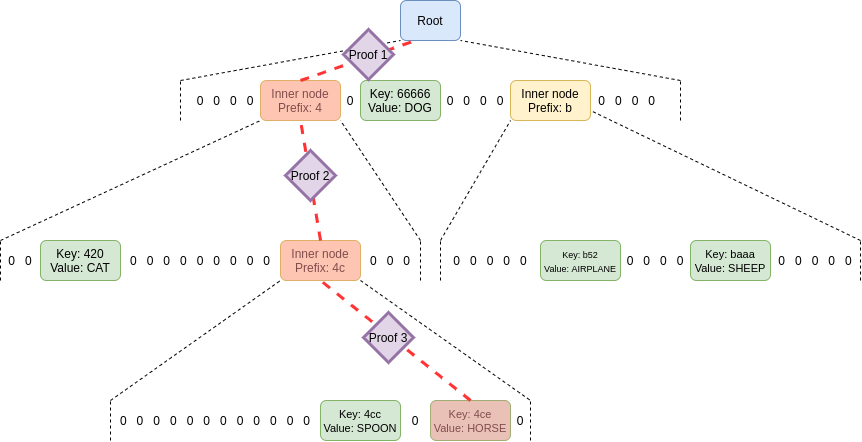
\includegraphics[width=\textwidth]{verkle_proof_animated.png}
    \end{center}
    % \textbf{Key Difference:} No sibling hashes needed! Polynomial commitment allows proving position $i$ contains value $v$ with constant-size proof regardless of tree width.
\end{frame}

\begin{frame}{8.3 Comparison: MPT vs Verkle Tree}
    \begin{columns}[t]
    \column{0.48\textwidth}
    \textbf{MPT:}
    \begin{itemize}
        \item Large witness size ($\sim$2 MB/block)
        \item Linear proof growth with siblings
        \item Not scalable for statelessness
        \item Proof size: $O(\log n \times b)$ where $b$ = branching factor
        \item Narrow branching (16) makes the path longer
    \end{itemize}
    
    \column{0.48\textwidth}
    \textbf{Verkle:}
    \begin{itemize}
        \item Small witness size ($\sim$100-200 KB)
        \item Doesn't depend on the size of the siblings
        \item Enables practical statelessness
        \item Proof size: $O(\log n)$ regardless of width
        \item Wider branching (256) makes the path shorter
    \end{itemize}
    \end{columns}
    
    % \vspace{0.3cm}
    % \textbf{Conclusion:} Verkle trees make stateless Ethereum feasible by reducing witness sizes by $\sim$20x, enabling nodes to verify blocks without storing full state.
\end{frame}
\end{document}